\documentclass{ximera}

\title{Trig Limits and Squeeze Theorem Activity Solution Guide}
\author{MATH 425: Calculus I}

\begin{document}
\begin{abstract}
    Working with the peers in your group, solve the following problems. Make sure to show and justify all your work. Make sure everyone in the group understands the solution and participates. Be prepared to report your answers to the whole class. 
\end{abstract}
\maketitle


\begin{exercise}
    Evaluate the limits.
    \begin{enumerate}
        \item $\displaystyle \lim_{x\rightarrow 0}\frac{\sin(7x)}{3x}$\\
        \textcolor{blue}{$=\lim_{x\rightarrow 0} \frac{\sin(7x)}{3x}\bigg(\frac{7}{7}\bigg)=\lim_{x\rightarrow 0}\frac{\sin(7x)}{7x}\bigg(\frac{7}{3}\bigg)=(1)\frac{7}{3}=\frac{7}{3}$}

        \item $\displaystyle\lim_{\theta \rightarrow 0}\frac{\sin(3\theta)\sin(5\theta)}{3\theta^2}$\\
        \textcolor{blue}{$=\lim_{\theta\rightarrow 0}\bigg(\frac{\sin(3\theta)}{3\theta}\bigg)\bigg(\frac{\sin(5\theta)}{\theta}\bigg)\frac{5}{5}=\lim_{\theta\rightarrow 0}5\bigg(\frac{\sin(3\theta)}{3\theta}\bigg)\bigg(\frac{\sin(5\theta)}{5\theta}\bigg)=5(1)(1)=5$}

        \item $\displaystyle\lim_{x\rightarrow 0} \frac{\cos(x)-1}{\tan(x)}$\\
        \textcolor{blue}{$=\displaystyle\lim_{x\rightarrow 0}\frac{\cos(x)-1}{\frac{\sin(x)}{\cos(x)}}=\lim_{x\rightarrow 0}(\cos(x)-1)\frac{\cos(x)}{\sin(x)}\bigg(\frac{x}{x}\bigg)$\\
    $=\displaystyle \lim_{x\rightarrow 0}\bigg(\frac{\cos(x)-1}{x}\bigg)\bigg(\frac{x}{\sin(x)}\bigg)\cos(x)=0(1)(1)=0$}

        \item $\displaystyle\lim_{x\rightarrow \pi^-} \ln(\sin(x))$ (Hint: a graph of $y=\ln(x)$ may be enlightening.)\\
        \textcolor{blue}{$\displaystyle\lim_{x\rightarrow \pi^-}\sin(x)=0$, but coming from the positive side. (Think of it as $f(x)\rightarrow 0^+$\\
        Then $\displaystyle\lim_{x\rightarrow 0^+}\ln(x)=-\infty$ (check on a graph if you don't understand how I got this.) \\
        Thus $\displaystyle\lim_{x\rightarrow \pi^-} \ln(\sin(x))=-\infty$}
    \end{enumerate}  
    
\end{exercise}

\begin{exercise}
  The indirect nature of the squeeze theorem can make it difficult to master.  Your group will review the squeeze theorem and use it to work out another indeterminate form which cannot be resolved in a direct fashion.\\

  The Squeeze Theorem (here I have chosen to use $L(x)$, $U(x)$ to notate the \textbf{lower} and \textbf{upper} bounding functions which are squeezing $f$): If $L(x)\leq f(x)\leq U(x)$ for all $x$ close to $c$, and \textbf{both} $\displaystyle \lim_{x\rightarrow c}L(x)=V$, and $\displaystyle\lim_{x\rightarrow c}U(x)=V$, then $\displaystyle\lim_{x\rightarrow c}f(x)=V$, as well.\\

  To use this theorem, we need an $f(x)$ which cannot be handled with direct evaluation or simplification, and then we need to find bounding functions $L$ and $U$ which satisfy the remaining requirements in the theorem.
  In the first exercise, we consider $$\lim_{x\rightarrow 0}\frac{x}{2^x-2}$$
  \begin{enumerate}
    \item First check that this is sufficiently nasty. (\textit{Direct evaluation should fail, and the limit should appear to be indeterminate.})\\
    \textcolor{blue}{subbing in $x=0$: $\frac{e^0-1}{0}=\frac00$ (indeterminate)}

    \item For the next part, consider the following functions: 
    $$g(x)=x^{\frac23},\;\;\;\;\;h(x)=-x^{\frac23}$$

    \item Graph all three of  these functions for $x$ values near zero. (Use technology, and verify that you have the correct setup for the squeeze theorem).\\
    \begin{image}
      \begin{tikzpicture}
  \begin{axis}[
    width=12cm,height=8cm,
    axis lines=middle,
    xlabel={$x$}, ylabel={$y$},
    xmin=-4, xmax=4,
    ymin=-4, ymax=4,
    samples=600,
    domain=-4:4,
    legend style={cells={anchor=west},at={(0.02,0.98)},anchor=north west},
    every axis x label/.style={at={(current axis.right of origin)}, anchor=west},
    every axis y label/.style={at={(current axis.above origin)}, anchor=south},
    grid=both,
    minor tick num=1
  ]

  % ---- Define helper functions ----
  % Real 2/3 power for all real x: |x|^(2/3)
  \pgfmathdeclarefunction{powTwoThirds}{1}{%
    \pgfmathparse{pow(abs(#1), 2.0/3.0)}%
  }

  % f(x) = x/(2^x - x)
  \pgfmathdeclarefunction{f}{1}{%
    \pgfmathparse{%
      (#1) / (pow(2, #1) - (#1))%
    }%
  }

  % ---- Plot f(x) with safeguards near singularities ----
  % We clip extreme y to keep the graph readable.
  \addplot[
    thick, blue,
    domain=-4:4,
    restrict y to domain=-4:4,
    unbounded coords=discard
  ]
  { f(x) };
  \addlegendentry{$f(x)=\dfrac{x}{2^x - x}$}

  % ---- Plot g(x) = x^(2/3) ----
  \addplot[
    very thick, red
  ]
  { powTwoThirds(x) };
  \addlegendentry{$g(x)=x^{2/3}$}

  % ---- Plot h(x) = -x^(2/3) ----
  \addplot[
    very thick, teal!60!black
  ]
  { -powTwoThirds(x) };
  \addlegendentry{$h(x)=-x^{2/3}$}

  % Optional: emphasize the axes ticks at integers
  \foreach \xx in {-4,-3,-2,-1,1,2,3,4}{
    \addplot[mark=*,mark size=0.7pt, only marks] coordinates {(\xx,0)};
  }
  \foreach \yy in {-4,-3,-2,-1,1,2,3,4}{
    \addplot[mark=*,mark size=0.7pt, only marks] coordinates {(0,\yy)};
  }

  \end{axis}
\end{tikzpicture}
    \end{image}

    \item Apply $\lim_{x\rightarrow 0}$ to the chain of inequalities, and appeal to the squeeze theorem to determine the value of this limit. \\
    \textcolor{blue}{$$\lim_{x\rightarrow0}1-x^{\frac23}\leq \lim_{x\rightarrow 0}\frac{e^x-1}{x}\leq \lim_{x\rightarrow 0}1+x^{\frac23}$$
    By the squeeze theorem, $\displaystyle\lim_{x\rightarrow 0}\frac{e^x-1}{x}=1.$}
  \end{enumerate}
\end{exercise}

\begin{exercise}
    The squeeze theorem can be hard to use on complicated problems in the wild.  Consider the following argument: \\
    A student is trying to determine the value of the limit: $$\lim_{x\rightarrow 0}\frac{x^2}{\sin(x)}.$$
    The student has discovered that when $x$ is close to zero, the following chain of inequalities is true: 
    $$\frac{x^3}{\sin(x)}\leq\frac{x^2}{\sin(x)}\leq\frac{x}{\sin(x)}.$$
    Discuss with your group how much knowledge you can gain from this chain of inequalities. (i.e. Is this chain enough to use the squeeze theorem?  Do these choices of $L(x)$ and $U(x)$ satisfy all of the requirements of the squeeze theorem?  Is there any information that can be extracted by applying a limit to this chain of inequalities? (Hint: Maybe we can establish what the limit \textbf{cannot} be, even if we don't know what it is yet.))\\
    \textcolor{blue}{This inequality does not satisfy the squeeze theorem, as $\lim_{x\rightarrow 0^+}\frac{x}{\sin(x)}=1$ and $\lim_{x\rightarrow 0^+}\frac{x^3}{\sin(x)}=0$. However, we can say that $0\leq \lim_{x\rightarrow 0^+}\frac{x^2}{\sin(x)}\leq 1$.}
     
\end{exercise}




\end{document}